\section{Relational Convolutions}\label{sec:relconv}

\subsection{Relational convolutions with discrete groups}
Suppose that we have a sequence of objects $(x_1, ..., x_n) \in (\mathbb{R}^{d})^m$ and a relation tensor $R \in \mathbb{R}^{n \times n \times d_r}$ describing the pairwise relations between them. $R$ should be thought of as obtained by a multi-head relation layer. The operation we will define does two things: 1) extracts relations between larger groups of objects using pairwise relations 2) transforms the relation tensor back into a sequence of objects, allowing it be composed with another relational layer.

Fix some filter size $s < n$, where $s$ is a hyperparameter of this grouping module/layer. One `filter' is given by the `graphlet' $f_1 \in \mathbb{R}^{s \times s \times d_r}$. This is a template for a `relation tensor' between $s$ objects. Note that the dimension of the relations in this filter matches that of the input relation tensor (i.e., the same $d_r$). Let $g \subset [n]$ be a subset of the objects $1, \ldots, m$ of size $s$. Suppose for now that $g$ is an ordered set (i.e., the group $(1, 2, 3)$ is different from the group $(2, 3, 1)$). Then, denote the relation tensor given by this (ordered) subset by $R[g] := [R[i,j]]_{i,j \in g}$. We define the relational inner product between this relation subtensor and the filter $f_1$ by
\begin{equation}
    \label{eq:relational_inner_prod_one_filt}
    \reliprod{R[g]}{f_1} \coloneqq \sum_{i,j \in g} \iprod{R[i,j]}{f_1[i,j]}_{\reals^{d_r}} = \sum_{i,j \in g} \sum_{k \in [d_r]} R[i,j,k] f_1[i,j,k].
\end{equation}

This is simply the inner product in the corresponding euclidean space $\mathbb{R}^{s^2 d_r}$ when each tensor is flattened. We call $\iprod{\cdot}{\cdot}_{\mathrm{rel}}$ the `relational inner product'. This quantity represents how much the relations within the objects in $g$ match the relations in the template $f_1$.

% Another relevant configuration is when the relation tensor $R$ is assumed to be symmetric (i.e.: pairwise relations are symmetric). In this case, filters can be restricted to be symmetric, and can now be identified with the smaller space $\{f \in \mathbb{R}^{s \times s \times r}: f[i,j] = f[j,i] \ \forall i,j \}$. The definition of the relational inner product can be simplified in this case to $\langle R[g], f_1 \rangle_R \coloneqq \sum_{i \leq j \in g} \langle R[i,j], f_1[i,j] \rangle$.

The relational convolution layer has some number of filters, $n_f$, which is also a hyper-parameters. Denote the collection of filters by $\boldsymbol{f} = \paren{f_1, \ldots, f_{n_f}} \in \reals^{s \times s \times d_r \times n_f}$, which we call a \textit{relational graphlet filter} (`relational' because it describes relations, `graphlet' because it corresponds to a subset of the $m$ objects, and filter because it is a template against which the relation tensor is compared). We define the relational inner product of a relation subtensor $R[g]$ with a relational graphlet filter $\bm{f}$ as the $n_f$-dimensional vector consisting of the relational inner products with each filter,
\begin{equation}
    \label{eq:relational_inner_prod}
    \reliprod{R[g]}{\bm{f}} \coloneq \begin{pmatrix} \reliprod{R[g]}{f_1} \\ \vdots 
 \\ \reliprod{R[g]}{f_{n_f}} \end{pmatrix} \in \mathbb{R}^{n_f}
\end{equation}

This vector summarizes various aspects of the relations within a group, captured by several different filters. We have overloaded notation, but will use the convention that a collection of filters is denoted by a bold symbol to distinguish between the two forms of the relational inner product. Each filter corresponds to one dimension in the final relation-summarizing vector for the group $g$. This is reminiscent of convolutional neural networks, where each filter gives us one channel in the output tensor.

We can also define a symmetric variant of the relational inner product which is invariant to the ordering of the elements in $g$. This can be done by pooling over all permutations of $g$. In particular, we suggest max-pooling and average-pooling, although any set-aggregator would be valid. We denote the permutation-invariant relational inner product by $\iprod{R[g]}{f_1}_{\mathrm{rel}, \mathrm{sym}}$,
\begin{equation}\label{eq:symmetric_relational_inner_prod}
    \iprod{R[g]}{\bm{f}} \coloneq \mathrm{Pool}\paren{\set{\reliprod{R[g']}{\bm{f}} \colon g' \in g!}},
\end{equation}
\noindent where $g!$ denotes the set of permutations of the group $g$. Recall that each $\iprod{R[g']}{\bm{f}}_{\mathrm{rel}}$ is $n_f$ dimensional, and the pooling is done independently for each dimension.

For a given group $g \subset [m]$, the relational inner product with a graphlet filter, $\iprod{R[g]}{\bm{f}}_\mathrm{rel}$, gives us a vector summarizing the relational patterns inside that group. We aim to get a sequence of objects which each describes the relational pattern within a particular group. Let $\calG$ be a set of size-$s$ groups of the the $m$ objects. The relational convolution between a relation tensor $R$ and a relational graphlet filter $\bm{f}$ is the sequence of relational inner products with each group in $\calG$,

\begin{equation}
    \label{eq:relational_convolution}
    R \ast \bm{f} \coloneq \left( \reliprod{R[g]}{\boldsymbol{f}} \right)_{g \in \calG} \equiv \left(z_1, ..., z_{\abs{\calG}}\right) \in (\mathbb{R}^{n_f})^{\abs{\calG}}
\end{equation}

$\calG$ is a pre-specified hyperparameter of the relational convolution operation. The choice depends on the usecase. If some prior information is known about reasonable groupings, this can be encoded in $\calG$. When $m$ is small and no prior information is available, a reasonable choice might be the the set of all combinations of size $s$. When $m$ is large, considering all combinations will be intractable. One solution which works well in practice is to consider a random sample of combinations. In the next subsections, we consider the problem of \textit{learning} the relevant groups.

One important advantage of the relational convolution operation is its interpretability. The filters $\bm{f} = (f_1, \ldots, f_{n_f})$ are each a particular pattern of relations between $s$ objects. Furthermore, each object in the relational convolution $R \ast \bm{f}$ represents the degree to which the relations in the group $g$ match the patterns in each filter.

In the above, we either consider all possible groups or we somehow assume that the relevant groups $\calG$ are known and given. We may also wish to \textit{learn} the relevant groups.

\begin{figure}[!ht]
    % \begin{tikzpicture}[node distance=2cm]


% parameters
\definecolor{highlightcolor}{rgb}{0.36, 0.54, 0.66}
\def\edgethickness{2}
\def\edgeOpacity{{30, 50, 70, 30, 50}}
\def\nodeColors{{"highlightcolor", "highlightcolor", "highlightcolor", "white", "white"}}
\def\graphsize{1.5}

% first graph
\begin{scope}[local bounding box=graph1]
    % Nodes
    \foreach \i in {1,...,5} {
        \pgfmathsetmacro\color{\nodeColors[\i-1]};
        \node[circle, draw, fill=\color] (N1\i) at (90+\i*72:\graphsize) {};
    }

    % Edges
    \foreach \i in {1,...,5} {
        \foreach \j in {1,...,5} {
            \ifnum\i<\j
                \pgfmathtruncatemacro\index{\i-1}
                \pgfmathsetmacro\opacity{\edgeOpacity[\index]}
                \draw[black!\opacity, line width=\edgethickness pt] (N1\i) -- (N1\j);
            \fi
        }
    }
\end{scope}

% second graph
\def\nodeColors{{"highlightcolor", "white", "highlightcolor", "highlightcolor", "white"}}
\begin{scope}[shift={(4,0)}, local bounding box=graph2]
    \foreach \i in {1,...,5} {
        \pgfmathsetmacro\color{\nodeColors[\i-1]};
        \node[circle, draw, fill=\color] (N2\i) at (90+\i*72:\graphsize) {};
    }
    % Edges
    \foreach \i in {1,...,5} {
        \foreach \j in {1,...,5} {
            \ifnum\i<\j
                \pgfmathtruncatemacro\index{\i-1}
                \pgfmathsetmacro\opacity{\edgeOpacity[\index]}
                \draw[black!\opacity, line width=\edgethickness pt] (N2\i) -- (N2\j);
            \fi
        }
    }
\end{scope}

% third graph
\def\nodeColors{{"white", "white", "highlightcolor", "highlightcolor", "highlightcolor"}}
\begin{scope}[shift={(10,0)}, local bounding box=graph3]
    \foreach \i in {1,...,5} {
        \pgfmathsetmacro\color{\nodeColors[\i-1]};
        \node[circle, draw, fill=\color] (N3\i) at (90+\i*72:\graphsize) {};
    }
    % Edges
    \foreach \i in {1,...,5} {
        \foreach \j in {1,...,5} {
            \ifnum\i<\j
                \pgfmathtruncatemacro\index{\i-1}
                \pgfmathsetmacro\opacity{\edgeOpacity[\index]}
                \draw[black!\opacity, line width=\edgethickness pt] (N3\i) -- (N3\j);
            \fi
        }
    }
\end{scope}

% graphlet filter
\def\triangleSize{1.5} % Set the desired size of the triangle
\begin{scope}[shift={(4,4)}, local bounding box=triangle]
    % nodes
    \foreach \i in {1,...,3} {
        \node[circle, draw] (T\i) at (90+\i*120:\triangleSize) {};
    }
    % edges
    \draw[black!80, line width=\edgethickness pt] (T1) -- (T2);
    \draw[black!40, line width=\edgethickness pt] (T1) -- (T3);
    \draw[black!30, line width=\edgethickness pt] (T2) -- (T3);
\end{scope}

\draw (T1) -- (graph1.north) node[midway] {$\iprod{\cdot}{\cdot}_\mathrm{rel}$};
\draw (triangle.south) -- (graph2.north) node[midway] {$\iprod{\cdot}{\cdot}_\mathrm{rel}$};
\draw (T2) -- (graph3.north) node[midway] {$\iprod{\cdot}{\cdot}_\mathrm{rel}$};
\path (graph2.east) -- (graph3.west) node[midway] {$\cdots$};

\node [minimum size=1cm, below=1cm of graph1.south] (tz1) {$\tilde{z}_1$};
\node [minimum size=1cm, below=1cm of graph2.south] (tz2) {$\tilde{z}_2$};
\node [minimum size=1cm, below=1cm of graph3.south] (tzng) {$\tilde{z}_{\abs{\calG}}$};

\draw (graph1.south) -- (tz1.north);
\draw (graph2.south) -- (tz2.north);
\draw (graph3.south) -- (tzng.north);

\node [minimum size=1cm, below right=1.5cm and 1cm of tz1.south] (z1) {$z_1$};
\node [minimum size=1cm, below=1.5cm of tz2.south] (z2) {$z_2$};
\node [minimum size=1cm, below left=1.5cm and 1cm of tzng.south] (zng) {$z_{n_g}$};
\path (tz2.east) -- (tzng.west) node[midway] {$\cdots$};

\draw (tz1.south) -- (z1.north);
\draw (tz1.south) -- (z2.north);
\draw (tz1.south) -- (zng.north);
\draw (tz2.south) -- (z1.north);
\draw (tz2.south) -- (z2.north);
\draw (tz2.south) -- (zng.north);
\draw (tzng.south) -- (z1.north);
\draw (tzng.south) -- (z2.north);
\draw (tzng.south) -- (zng.north);
\path (z2.east) -- (zng.west) node[midway] {$\cdots$};

\node [left=0.1cm of graph1.west, align=center] (relsubtensors) {relation subtensors\\ $R[g],\, g \in \calG$};
\node [left=of tz1, below=6.5em of relsubtensors] (relconv) {$R \ast \bm{f}$};
\node [left=of z1, below=5.25em of relconv] (relconvsoft) {$(R \ast \bm{f})(G)$};
\node [left=of triangle, above=8em of relsubtensors,  align=center] (filters) {graphlet filters \\ $\bm{f} \in \reals^{s \times s \times d_r \times n_f}$};

\end{tikzpicture}
    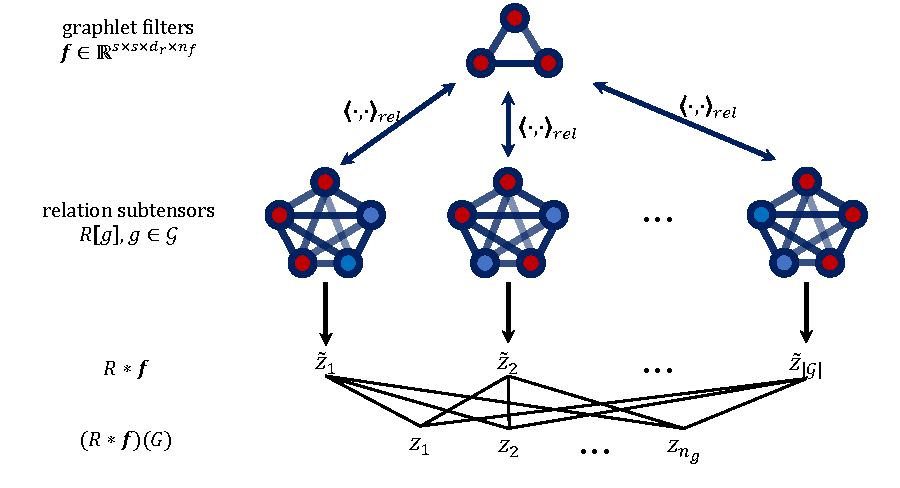
\includegraphics[width=\textwidth]{figs/relconv_diagram2.pdf}
    \caption{A depiction of the graphlet relational convolution operation. The input is a relation tensor $R$ of shape $m \times m \times d_r$, giving pairwise relations of dimension $d_r$ between a sequence of $m$ objects. A graphlet filter of size $s$ is parameterized by a relation tensor of shape $s \times s \times d_r$. The graphlet convolution operation computes relational inner products for each of $n_f$ graphlet filters, $\bm{f}$. This gives a vector representation, $z_i \in \reals^{n_f}$, for each discrete group of $s$ objects. Finally, this is synthesized into a vector representation for each of $n_g$ `soft groups', $G$. The overall operation is denoted by $(z_1, \ldots, z_{n_g}) = (R \ast \bm{f})(G)$.}\label{fig:relconvdiagram}
\end{figure}


\subsection{Relational convolutions with `soft' groups}

In the above formulation, the groups are `discrete', and we consider every possible group. Having discrete groups can be nice for interpretability. But, one challenge we face here is that the number of objects grows rapidly after applying this module. That is, the number of groups to consider $\abs{\calG} = \binom{m}{s}$ may be intractably large, especially if the number of input objects $n$ is large. This may pose computational issues. Furthermore, considering every possible grouping may be unnecessary and may make learning more difficult.

In order to address these issues, we might want to explicitly model the groups. This allows us to control the number of objects in the output sequence such that only useful groups are considered.

In the next section, we outline some ways to model `soft groups' using \textit{Grouping Layers}. These layers take a sequence of objects and/or the relation tensor as input and produce a group matrix $G \in \reals^{m \times n_g}$ representing $n_g$ `soft groups'. The $(i,j)$th entry of the group matrix represents the degree to which the $i$th object belongs to the $j$th group. The number of groups $n_g$ is a configurable hyperparameter of the grouping layers. The groups may be a function of the position of the objects in the sequence, the features of the objects, and/or the relations between objects. Different grouping schemes may be more or less appropriate for different tasks. This is discussed in detail in the next section. For now, we assume that the group matrix $G$ is given as input the relational convolution layer.

Consider the group matrix $G \in \reals^{m \times n_g}$ and filters $\bm{f}$ of size $s$. First, we use $G$ to compute a ``group-match score'' for each discrete group $g$ of size $s$ (e.g., $g \in \calG = \binom{[m]}{s}$). This is done via

\begin{equation}
    \label{eq:group_match_score}
    \begin{split}
        G &\gets \text{SoftPlus}(G)\\
        \alpha_{gk} &\gets \text{Softmax}\paren{\paren{\prod_{i \in g} G[i,k]}_{g \in \calG}}, \quad g \in \calG, k \in [n_g],
    \end{split}
\end{equation}

where the soft-plus function is $\text{Softplus}(x) = \log(\exp(x + 1))$, applied elementwise. This has the effect of making the group matrix $G$ non-negative which is needed for the product of its elements to represent a ``group-match score''. The product inside the softmax is over elements in the discrete group $g \in \calG$. Hence, it will be large whenever the softgroup $G[:, k]$ aligns with the discrete group $g$. Thus, $\alpha_{gk}$ is a normalized ``group-match score'' indicating the degree to which the discrete group $g$ matches the given soft group $G[:,k]$. Note that the group match scores of discrete groups sum to one: $\sum_{g \in G} \alpha_{gk} = 1, \ \forall k \in [n_g]$.

Now, we can define the `soft' relational inner product given the `soft' group $G_k = G[:, k]$ by
\begin{equation}
    \label{eq:soft_relational_inner_prod}
    \langle R, \boldsymbol{f} \, \vert \, G_k \rangle_R \coloneqq \sum_{g \in \calG} \alpha_{gk} \iprod{R[g]}{\boldsymbol{f}}_\mathrm{rel}
\end{equation}

This notation should be read as ``the relational inner product of the relation tensor $R$ with the graphlet filters $\boldsymbol{f}$ given the group $G_k$''. This expression is essentially a convex combination of the relational inner product with all possible discrete groups weighted by how much they match the soft group $G_k$.

With this modification, the number of objects in the output sequence is fixed and controlled by the number of groups, $n_g$ (which is a hyperparameter). The output sequence of the relational convolution given groups $G$ is now given by

\begin{equation}
    \label{eq:soft_relational_convolution_groups}
    (R \ast \bm{f})(G) = \left( \softreliprod{R}{\bm{f}}{G_1}, \ldots, \softreliprod{R}{\bm{f}}{G_{n_g}} \right) \in \left(\mathbb{R}^{n_f}\right)^{n_g}
\end{equation}

\texttt{TODO: is this notation good?}

\subsection{Efficiency of `convolutions'}
The operation we have defined here is a `convolution' in the sense that we take a patch of the relation tensor, given by a group, and compare the relations within it to a template graphlet filter via an appropriately-defined inner product. This is similar to how, in a convolutional neural network, we would take a patch of an image and compare it to an image filter. Another similarity to CNNs is that the same graphlet filters are used for all groupings, thus enabling weight-sharing. This is similar to how the same convolutional filters are used for all image patches in a CNN. This makes our framework quite efficient when it comes to the number of parameters and, hopefully, makes learning easier.

% This connection extends to (message-passing) graph neural networks. A key difference however is the following. In a graph neural network, we compute a convolution \textit{along} the graph (i.e.: the graph is what determines a node's neighbors for message-passing). What we are proposing here is that we `convolve' the (relational) graph itself with another graph. 

This analogy motivates one possible style of architectures in our framework~\Cref{fig:relational_framework}. Namely, to have the number of groups after each relational-grouping module decrease while increasing the number of filters. This can be done until we obtain a single group with a long feature vector. This should give a representation of the relational features across all objects, including higher-order relational features (i.e., relations on relations). This single vector can then be passed to a dense feedforward network. This is similar to the ``fully convolutional network'' architecture, where the height and width of the tensor are iteratively decreased (by pooling layers) while increasing the number filters, resulting in a long and thin vector.

